%----------------------------------------------------------------------------------------
%	SECTION 1.1
%----------------------------------------------------------------------------------------

\section{Simple Cryptosystems and Classical Ciphers.}
\label{section1}

\begin{definition}
    We define a \textbf{cryptosystem} to be a triple $(\Pc, \Cc, \Kc)$ where
    $\Pc$ and  $\Cc$ are called the \textbf{plain text space} and
    \textbf{cipher text space}; and $\Kc$, called the \textbf{key space} is such
    that, for any $K \in \Kc$, there exist maps $e_K:\Pc \rightarrow \Cc$, and
    $d_K:\Cc \rightarrow \Pc$ such that $d_Ke_K(x)=x$ for every $x \in \Pc$. We
    call the elements of  $\Pc$ \textbf{plain texts}, the elements of $\Cc$
     \textbf{cipher texts}, and the elements of $\Kc$  \textbf{keys}. We call
     $e_K$ and  $d_K$ the  \textbf{encryption rule} and \textbf{decryption
     rule}, respectively. We call the pait $(e_K,d_K)$ the \textbf{cipher}.
\end{definition}
\begin{remark}
    It is important to note, that in this definition, we take $\Pc$ and $\Cc$ to
    be arbitrary sets. However, in practice, they will usually result to be
    vector spaces of fields like  $\F_2$. Recall that with computers, if we
    encrypt a message like \lstinline{Hello, world!}, we are encrypting a string
    of bits.
\end{remark}
\begin{remark}
    The property that $d_Ke_K(x)=x$ just implies that $e_K$ is the right inverse
    of  $d_K$. This howver, does not assert that  $e_K=\inv{d_K}$.
\end{remark}

The figure below outlines a communications channel between two parties Alice and
Bob. Here, Alice and Bob both agree on a protocol that uses a specified
cyrptosystem. They take a key $K$ from the set  $\Kc$ of the system. This key
then used by the ecnryptor, and by the decryptor  (through a secure channel) to
encrypt and decrypt messages.

\begin{figure}
    \centering
    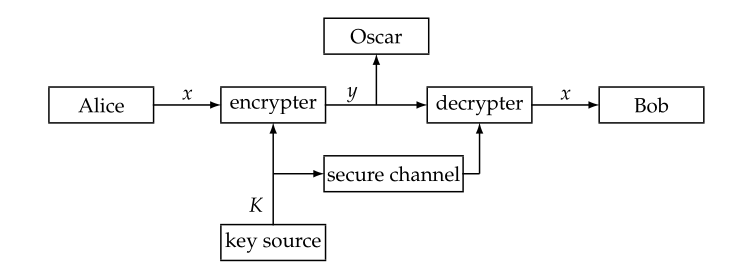
\includegraphics[scale = 0.5]{Figures/Chapter1/encrypt_comm_channel.png}
    \caption{Encrypted Communication Channel between Alice and Bob.}
    \label{fig_1.1}
\end{figure}

Oscar, who can intercept their encrypted
communications cannot read them without the key. For this reason, it is
important to choose the key $K$ in a secure setting. Here, the encyrptor and the
decryptor are just simply the maps $e_K$ and  $d_K$ of the system. We call this
kind of scheme a \textbf{symmetric key encryption protocol}, and we call the key
$K$ in this setting the  \textbf{symmetric key}, or the \textbf{secret key}.

\begin{lemma}\label{1.1.1}
    In any cryptosystem with any key $K$, the map $e_K$ is $1-1$.
\end{lemma}
\begin{proof}
    Let  $e=e_K$, and let  $x,y \in \Pc$ be such that  $e(x)=e(y)=z$. Then let
    $d=d_K$. Then $d(z)=d(e(x))=x$ and $d(z)=d(e(y))=y$, implying that $x=y$.
\end{proof}

\begin{lemma}\label{1.1.2}
    In any cryptosystem, if $\Pc=\Cc$, then  $e_K$ is a permutation on $\Pc$.
\end{lemma}
\begin{proof}
    We have that $e_K$ is  $1-1$. We have that $e_K(\Pc) \subseteq \Pc$. Now,
    let $x \in \Pc$, and consider $d_K(x)=y$. By definition, we get that
    $x=e_K(y)$ for some $y \in \Pc$. This makes $e_K(\Pc)=\Pc$, and hence onto.
    Therefore, $e_K$ is a permutation.
\end{proof}

We now finish the section by discribing the shift cipher.

\begin{definition}
    Let $\Pc=\Cc=\Kc=\faktor{\Z}{n\Z}$. We define the \textbf{shift cipher} to
    be the pair $(e_K, d_K)$, defined by the rules $e_K:x \rightarrow (x+K)
    \mod{26}$, and $d_K:y \rightarrow y-K \mod{n}$.
\end{definition}
\begin{remark}
    When $K=3$, we call the shift cipher the \textbf{Caesar cipher}.
\end{remark}

\begin{example}
    Let $Q=\{A,B,C, \dots, Z\}$ be the entire english alphabet. We implement the
    shift cipher on $Q$ by first taking the map  $Q \rightarrow \faktor{\Z}{26\Z}$
    defined by $A \rightarrow 0, B \rightarrow 1, C \rightarrow 2 \dots Z
    \rightarrow 25$; see figure \ref{fig_1.2} Then if $x$ is any English plain text
    message  (without spaces), we compute the cipher text on the image of $x$, and
    then take the inverse map to get our cipher  $y$ in English plaintext. To
    decrypt, it is the same process, except computing $d_K$.
\end{example}

\begin{figure}
    \centering
    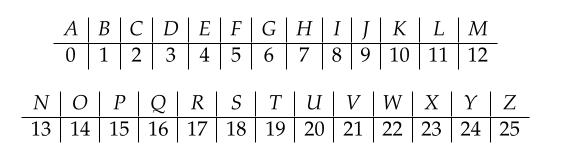
\includegraphics[scale = 0.5]{Figures/Chapter1/alpha_to_num.png}
    \caption{The mapping of $Q$ onto  $\faktor{\Z}{26\Z}$.}
    \label{fig_1.2}
\end{figure}

\begin{example}
    Using the shift cipher for $n=26$, choose the key $K=11$, and the plaintext
    message \lstinline{wewillmeetatmidnight}. Using the map $Q \rightarrow
    \faktor{\Z}{26\Z}$, we get the following:
    \begin{align*}
        22 && 4 && 8 && 22 && 11 && 11 && 12 && 4 && 4 && 19 \\
        0 && 19 && 12 && 8 && 3 && 13 && 8 && 6 && 7 && 19 \\
    \end{align*}
    Using the shift cipher, $\mod{11}$, we get the following:
    \begin{align*}
        7 && 15 && 7 && 19 && 22 && 22 && 23 && 15 && 15 && 4 \\
        11 && 4 && 23 && 19 && 14 && 24 && 19 && 17 && 18 && 4 \\
    \end{align*}
    So taking $\faktor{\Z}{26\Z} \rightarrow Q$, we get our cipher text to be:
    \lstinline{HPHTWWXPPELEXTOYTRSE}. To decrypt, we simply just reverse the
    process.
\end{example}

Normally, it is necessary to provide an intermediary map, such as the map $Q
\rightarrow \faktor{\Z}{26\Z}$ so that our plaintext can be computed to sipher
text. We call these maps \textbf{encodings}.

\begin{theorem}\label{1.1.3}
    Let $\Pc=\Cc=\Kc=\faktor{\Z}{n\Z}$, for any $K \in \Kc$, the shift cipher
    defines a cryptosystem.
\end{theorem}
\begin{proof}
    let $(e_K,d_K)$ be the encryption and decryption rules defined by the
    shift cipher for any $K \in \Kc$. That is $e_K(x)=x+K \mod{n}$ and
    $d_K(y)=y-K \mod{n}$, for any $x,y \in \Pc$. Thus, letting  $y=e_K(x)$, we
    get $d_K(y)=y-K \mod{n}=(x+K)-K \mod{26}=x+(K-K) \mod{n}=x \mod{n}$.
    Therefore, the pair $(e_K,d_K)$ define a cryptosystem.
\end{proof}

\begin{definition}
    We define a cyptosystem to be of \textbf{practical use} if:
    \begin{enumerate}
        \item[(1)] The ecnryption and decryption rules $e_K$ and  $d_K$ are
            computationally feasable; i.e. a anyone should be able to
            efficiently compute them.

        \item [(2)] An adversary obtaining a cipher text $y$ cannot determine
            the plaintext $x$, nor the key  $K$ in any computationally feasable
            ammount of time.
    \end{enumerate}
\end{definition}

\begin{example}
    The shift cipher is not of practical use. Notice that if we have any cipher
    text, we can simply try the following sequence $\{d_i\}_{i=0}^{25}$ of
    decryption rules until we successfully decrypt the cipher. For example, if
    we have the cipher text \lstinline{JBCRCLQRWCRVNBJENBWRWN} we dectypt it
    with the above sequence to obtain:
    \begin{verbatim}
                        jbcrclqrwcrvnbjenbwrwn
                        iabqbkpqvbqumaidmavqvm
                        hzapajopuaptlzhclzupul
                        gyzozinotzoskygbkytotk
                        fxynyhmnsynrjxfajxsnsj
                        ewxmxglmrxmqiweziwrmri
                        dvwlwfklqwlphvdyhvqlqh
                        cuvkvejkpvkogucxgupkpg
                        btujudijoujnftbwftojof
                        astitchintimesavesnine
    \end{verbatim}
    to obtain the plain text \lstinline{astitchintimesavesnine}. We notice that
    this was done in precisely $9$ computations. On average, we can compute the
    plaintext in $\frac{26}{2}=13$ computations.
\end{example}

\begin{definition}
    Let $\Pc=\Cc=\faktor{\Z}{n\Z}$ and let $\Kc=S_n$ the permutation group
    on $26$ elements. For $\pi \in \Kc$, we define the  \textbf{substitution
    cipher} on $\pi$ to be the pair $(e_{\pi}, d_{\pi})$ such that
    $e_{\pi}:x \rightarrow \pi(x)$ and $d_{\pi}:y \rightarrow \inv{\pi}(y)$.
\end{definition}

\begin{theorem}\label{1.2.1}
    For $\Pc=\Cc=\faktor{\Z}{n\Z}$ and any $\pi \in S_{26}$, the substitution
    cipher defines a cryptosystem.
\end{theorem}
\begin{proof}
    For any  $x, y \in \faktor{\Z}{n\Z}$, and $\pi \in S_n$, let
    $y=e_{\pi}(x)$. Then $d_{\pi}(y)=\inv{\pi}(e(x))=\inv{\pi}\pi(x)=x$.
\end{proof}

\begin{example}
    Let $\pi$ be the permutation defining the encryption rule $e=\pi$ by:
        \begin{verbatim}
            a b c d e f g h i j k l m n o p q r s t u v w x y z
            X N Y A H P O G Z Q W B T S F L R C V M U E K J D I
        \end{verbatim}
    and the decryption rule $d=\inv{\pi}$ by:
        \begin{verbatim}
            A B C D E F G H I J K L M N O P Q R S T U V W X Y Z
            d l r y v o h e z x w p t b g f j q n m u s k a c i
        \end{verbatim}
    Where, for $e$, the first row represents the elements $x \in
    \faktor{\Z}{26\Z}$, and the the second row represents the elements $e(x) \in
    \faktor{\Z}{26\Z}$. Likewise, for $d$, the first row represents all  $y$ and
    the second all  $d(y)$.

    Now take the cipher text:
        \begin{verbatim}
                    MGZVYZLGHCMHJMYXSSFMNHAHYCDLMHA
        \end{verbatim}
    we get the plain text:
        \begin{verbatim}
                    thisciphertextcannotbedecrypted
        \end{verbatim}
\end{example}

\begin{lemma}\label{1.1.5}
    Let $|\Pc|=\Cc|=n$. There are $n!$ possible keys for the substitution
    cipher.
\end{lemma}
\begin{proof}
    Notice a key in the substitution cipher is any permutation $\pi:\Pc
    \rightarrow \Cc$, hence there are $n!$ of them.
\end{proof}
\begin{remark}
    With the number of possible keys for the substitution cipher being $n!$, for
     $n$ sufficiently large, the permutations become dificult to count. For
     example, for $n=26$, there are already  $26!$ possible keys, which makes it
     infeasible to guess by brute force. This provides more secruity than the
     shift cipher, however there are other methods of breaking the substitution
     cipher.
\end{remark}

\begin{example}
    Shift ciphers are substitution ciphers.
\end{example}

Now, before defining the next cipher, lets state and prove a theorem from number
theory.

\begin{theorem}\label{1.1.6}
    Let $a,b \in \faktor{\Z}{n\Z}$. The congruence $ax \equiv b \mod{n}$ has
    unique solution for $x \in \faktor{\Z}{n\Z}$ if, and only if $(a,n)=1$.
\end{theorem}
\begin{proof}
    First suppose that $(a,n)=d>1$. Then the congruence $ax \equiv 0 \mod{n}$
    has two solutions $x=0$ and  $x=\frac{n}{d}$. This proves the first
    direction.

    Now suppose $(a,n)=1$. Then there exist $u, v \in \faktor{\Z}{n\Z}$ for
    which $au+vn \equiv au \equiv 1 \mod{n}$, thus $x = (au)x \equiv bu
    \mod{n}$. So $x=bu$ is a solution, that  $x$ is unique follows from the fact
    that  $u$ and  $v$ are uniquely determined.
\end{proof}
\begin{corollary}
    The congruence $ax+b \equiv y \mod{n}$ has unique solution if, and only if
    $(a,n)=1$.
\end{corollary}
\begin{remark}
    Here, the pair $(a,n)$ is taken to mean the greated common divisor of $a$
    and  $n$. Also note that if we consider this theorem group theoretically, we
    have $a \in U(\faktor{\Z}{n\Z})$, and the theorem reduces to the
    cancellation law for this group.
\end{remark}

\begin{definition}
    Let $\Pc=\Cc=\faktor{\Z}{n\Z}$ and let $K=U(\faktor{\Z}{n\Z})$. We define
    the \textbf{affine cipher} to be a substitution cipher defined by the pair
    $(e,d)$ where $e:x \rightarrow ax+b \mod{n}$ and $d:y \rightarrow
    \inv{a}(y-b) \mod{n}$.
\end{definition}

\begin{example}
    \begin{enumerate}
        \item[(1)] For the pair $(1,b)$, the affine cipher is equivalent to the
            shift cipher whos key is $b$.

        \item[(2)] For $n=26$ and the pair $K=(7,3)$ take $e(x)=7x+3 \mod{26}$
            and $d(y)=15(y-3) \mod{n} \equiv 15y-19 \mod{26}$. Then if $y=e(x)$,
            $d(y)=15(7x+3)-19 \equiv x+ (19-19) \equiv x \mod{n}$.
    \end{enumerate}
\end{example}

\begin{lemma}\label{1.1.7}
    The affine cipher defines a cryptosystem.
\end{lemma}

All these cryptosystem presented so far have one thing in common.

\begin{definition}
    We call a cryptosystem is said to be \textbf{monoalphabetic} if for any
    given key $K$, the encryption and decryption rules  $e_K$ and  $e_K$ map
    each element of  $\Pc$ to a unique element of $\Cc$ and viceversa.
\end{definition}

\begin{example}
    \begin{enumerate}
        \item[(1)] The shift cipher is monoalphabetic.

        \item[(2)] They cryptosystem defined by the substitution cipher is
            monoalphabetic; indeed since the key $\pi$ is a permutation, then it
            is  $1-1$ and onto, since  $e=\pi$,  $d=\inv{\pi}$, this establishes
            the result.

        \item[(3)] Affine ciphers are monoalphabetic, since they are
            substitution ciphers.
    \end{enumerate}
\end{example}

\begin{definition}
    Let $m \in \Z^+$, and let  $\Pc=\Cc=\Kc=(\faktor{\Z}{n\Z})^m$. Then for any
    $K=(k_1, \dots, k_m) \in (\faktor{\Z}{n\Z})^m$, define the pair $(e_K,d_K)$
    by the maps $e_K:x \rightarrow x+K \mod{m}$ and $d_kK:y \rightarrow y-K
    \mod{n}$, for $x=(x_1, \dots, x_m), y=(y_1, \dots, y_m) \in
    (\faktor{\Z}{n\Z})^m$. We call this cipher \textbf{Vigen\`ere's cipher}.
\end{definition}

\begin{theorem}\label{1.1.8}
    Vigen\`ere's cipher defines a cryptosystem.
\end{theorem}
\begin{proof}
    Let $x=(x_1, \dots, x_m)$ and $y=(y_1, \dots, y_m)$. Notice that $y=x+K
    \mod{n}$ if, and only if $y_i=x_i+k_i \mod{n}$. Thus each $k_i$ defines the
    key for a shift cipher, so we can see that when $y=e(x)$, then $d(y)=x$.
\end{proof}

\begin{example}
    Vigen\`ere's cipher is not monoalphabetic. Notice that the map $x+K
    =(x_i+k_i, \dots, x_m+k_m)$. Since each $x_i \in \faktor{\Z}{n\Z}$, and each
    $k_i$ is the key for a shift cipher, the map  $e(x)=x+K \mod{n}$ does not
    map elements of $\Pc$ uniquely.
\end{example}

\begin{figure}
    \centering
    \begin{verbatim}
                    thiscr yptosy stemis notsec ure
                    CIPHER CIPHER CIPHER CIPHER CIP
                    ------ ------ ------ ------ ----
                    VPXZGI AXIVWP UBTTMJ PWIZIT WZT

                    VPXZGI AXIVWP UBTTMJ PWIZIT WZT
                    YSLTWP YSLTWP YSLTWP YSLTWP YSL
                    ------ ------ ------ ------ ----
                    thiscr yptosy stemis notsec ure
    \end{verbatim}
    \caption{Encryption and decryption with Vigen\`ere's cipher. See example
    $(1.9)$.}
    \label{fig_1.3}
\end{figure}

\begin{example}
    Let $m=6$, and choose the key $K$ to be the word \lstinline {CIPHER}, so
    that with the map $Q \rightarrow \faktor{\Z}{26\Z}$, $K=(2,8,15,7,4,17)$. If
    we have the plain text:
         \begin{verbatim}
                    thiscryptosystemisnotsecure
        \end{verbatim}
    then we divide the plaintext into blocks of $6$ to get:
         \begin{verbatim}
                    thiscr yptosy stemis notsec ure
        \end{verbatim}
    treating each block as a $6$-tuple, i.e.
    \lstinline{thiscr}$=(19,7,8,18,2,17)$ (and \lstinline{ure}$=(20,17,4,0,0,0)$
    where we discard the remaining $3$ components), we can apply Vigen\`ere's
    cipher on each individual block to reviece the cipher blocks:
         \begin{verbatim}
                    VPXZGI AXIVWP UBTTMJ PWIZIT WZT
        \end{verbatim}
    We then concatenate each block to obtain the ciphertext:
         \begin{verbatim}
                    VPXZGIAXIVWPUBTTMJPWIZITWZT
        \end{verbatim}
    We can visualize this process in figure \ref{fig_1.3}. Decryption is the
    same process.
\end{example}

The cipher of Vigen\`ere has the property that given a keyword of length $m$, an
alphabetic character can be mapped onto one of  $m$ possible characters.

\begin{definition}
    Let $m \in \Z^+$. We call a cryptosystem  \textbf{polyalphabetic} if given a
    keyword of length $m$, of  $m$ distinct characters, then a given element of
     $\Pc$ can be mapped to any one of  $m$ possible elements of  $\Cc$.
\end{definition}

We now describe a cryptosystem that takes as plaintext a string of characters
and outputs a permutation on those characters.

\begin{definition}
    Let $\Pc=\Cc=(\faktor{\Z}{n\Z})^m$ and let $\Kc=S_m$ We define the
    \textbf{transpostion cipher} (or \textbf{permutation cipher}) to be a pair
    $(e_{\pi},d_{\pi})$, for $\pi \in S_m$ such that for any  $x,y \in
    (\faktor{\Z}{n\Z})^m$, $e_{\pi}(x)=(x_{\pi(1)}, \dots x_{\pi(m)})$ and
    $d(y)=(y_{\inv{\pi}(1)}, \dots, y_{\inv{\pi}(m)})$.
\end{definition}

\begin{theorem}\label{1.1.9}
    The transposition cipher defines a cryptosystem.
\end{theorem}
\begin{proof}
    Let $\pi \in S_m$ and $y=e_{\pi}(x)=(x_{\pi(1)}, \dots x_{\pi(m)})$. Then
    $d(y)=(x_{\inv{\pi}(\pi(1))}, \dots x_{\inv{\pi}(\pi(m))})=(x_1, \dots,
    x_m)=x$.
\end{proof}

\begin{example}
    Let $m=6$,  $n=26$ and define  $\pi \in S_m$ by the permutation  $\pi=(1 \
    3)(2 \ 5 \ 4 \ 6)$. Then $\inv{\pi}=(1 \ 3)(6 \ 4 \ 5 \ 2)$. Given the
    plaintext:
    \begin{verbatim}
                        shesellseashellsbytheseashore

    \end{verbatim}
    Encryption is proceeds similarly as in Vigen\`ere's cipher. We partition the
    message into blocks of $6$:
    \begin{verbatim}
                        shesel lsseas hellsb ythese ashore
    \end{verbatim}
    Then apply the encryption rule $e_{\pi}(x)=(x_{\pi(1)}, \dots x_{\pi(m)})$
    to get the cipher blocks:
    \begin{verbatim}
                        EESLSH SALSES LSHBLE HSYEET HRAEOS
    \end{verbatim}
    and we then concatenate the blocks to obtain the ciphertext:
    \begin{verbatim}
                        EESLSHSALSESLSHBLEHSYEETHRAEOS
    \end{verbatim}
    Decryption is the same, except we use $d_\pi$ instead of  $e_\pi$ on the
    ciphertext.
\end{example}

So far, the ciphers presented all (with exception of Vigen\`ere's cipher) use
one key to ecnrypt the whole message. These kind of ciphers encrypt the message
in ``blocks''. However, this isn't the only way to excrypt messages.

\begin{definition}
    We call the cipher $(e,d)$ of a given cryptosystem a \textbf{block cipher}
    if successive plaintext elements $x \in \Pc$ are encrypted using the same
    key  $K \in \Kc$; that is, for any cipher text string  $y=y_1 \dots y_m$ of
    length $m$,  $y=e(x_1) \dots e(x_m)$ where $x=x_1 \dots x_m$ is the
    associated plaintext string.
\end{definition}
\begin{remark}
    When we say string, we simply mean an $m$-tuple of elements. We can then
    alternatively write  $x=x_1x_2 \dots x_m$ to denote $x=
    (x_1, x_2, \dots, x_m)$. We will often write tuples this way when we want to
    emphasize them as being strings, or some other symbol stream.
\end{remark}

\begin{example}
    The shift, substitution, and transposition ciphers are all block ciphers.
\end{example}

We now define a type of cipher that is not a block cipher.

\begin{definition}
    Let $\Pc$, and $\Cc$ be finite plaintext and ciphertext spaces,
    respectively, and let $\Kc$ be a finite key space. let  $\Lc$ be a finite
    set called the  \textbf{key stream alphabet}. We define the
    \textbf{synchronous stream cipher} as follows: define the map $g:\Kc
    \rightarrow \Lc^m$, where $m \in \Z^+$, called the \textbf{key stream
    generator}, such that $g:K \rightarrow z=z_1z_2 \dots z_m$. Then define the
    pair $(e_z,d_z)$ for each $z \in \Lc$ such that $e_z:\Pc \rightarrow \Cc$
    and $d_z:\Cc \rightarrow \Pc$ with $d_z(e_z(x))=x$. We call elements of
    $\Lc^m$  \textbf{keystreams}.
\end{definition}
\begin{remark}
    When $m \in \Z^+$, we call the stream cipher  \textbf{finite}, and the
    keystream $z$ a  \textbf{finite keystream}. Often however, we want infite
    keystreams. To do this, we just take $m>M$ for some arbitrarily large  $M
    \in \Z^+$; we then call  $z$ an  \textbf{infinite keystream} and we call the
    stream cipher infinite.
\end{remark}

\begin{example}
    \begin{enumerate}
        \item[(1)] Vigen\`ere's cipher is a finite synchronous stream cipher.
            Let $m \in \Z^+$ be the length of a given keyword  $K=
            (k_1, \dots, k_m)$. Let $\Pc=\Cc=\Lc=\faktor{\Z}{26\Z}$ and
            $\Kc=(\faktor{\Z}{26\Z})^m$. Define then the pair $(e_z,d_z)$ such
            that $e_z:x \rightarrow x+z \mod{26}$ and $d_z:y \rightarrow y-z
            \mod{26}$, where $z=z_1 \dots z_m$ and each
            $z_i=\begin{cases}
                    k_i,    & 1 \leq i \leq m \\
                    z_i-m,  & i \geq m+1 \\
                 \end{cases}$.

         \item[(2)] Block ciphers are finite stream ciphers where the keystream
             consist of characters $z_i=K$ for all  $1 \leq i \leq m$; i.e. the
             keystream is constant.
    \end{enumerate}
\end{example}

\begin{definition}
    We call a stream cipher \textbf{periodic} with period $d$ if for some
    keystream  $z$,  $z_{i+d}=z_i$ for all $i \geq 1$. We write  $\ord{z}=d$.
\end{definition}

\begin{example}
    Defining Vigen\`ere's cipher as an infinite stream cipher, it is periodic
    with period $\ord{z}=m$.
\end{example}

Often with stream ciphers, we have that $\Pc=\Cc=\Lc=\faktor{\Z}{2\Z}$. This
motivates us to define a method for creating keystreams.

\begin{definition}
    Let $m \in \Z^+$, and let  $z=(z_1, \dots, z_m) \in (\faktor{\Z}{n\Z})$. We
    call $z$ a  \textbf{linear recurrence} of degree $\deg{z}=m$ if
    \begin{equation}
        z=\sum_{j=0}^{m-1}{c_jz_{i+j}} \mod{n}
    \end{equation}
    for all $i \geq 1$, and where  $c_j \in \faktor{\Z}{n\Z}$ for $1 \leq j \leq
    m-1$ are called the \textbf{constants} of the linear recurrence.
\end{definition}
\begin{remark}
    Often we use linear recurrences when working with $n=2$.
\end{remark}

One appealing aspect of using linear recurrence with binary messages (i.e. in
$\faktor{\Z}{2\Z}$) is that they can be easily implemented in harware using
linear feedback shift registers; which we define abstractly as:

\begin{definition}
    We define a \textbf{linear feedback shift register} of $m$ \textbf{steps} to
    be a set of rules: for some keystream $k=(k_1, \dots k_m) \in
    (\faktor{\Z}{2\Z})^m$,
    \begin{enumerate}
        \item[(1)] $k_1$ is the next  keystream bit.

        \item[(2)] $k_2, \dots k_m$ is shifted one stage left.

        \item[(3)] $k_m=\sum_{j=0}^{m-1}{c_jk_{j+1}}$
    \end{enumerate}
\end{definition}

\begin{figure}
    \centering
    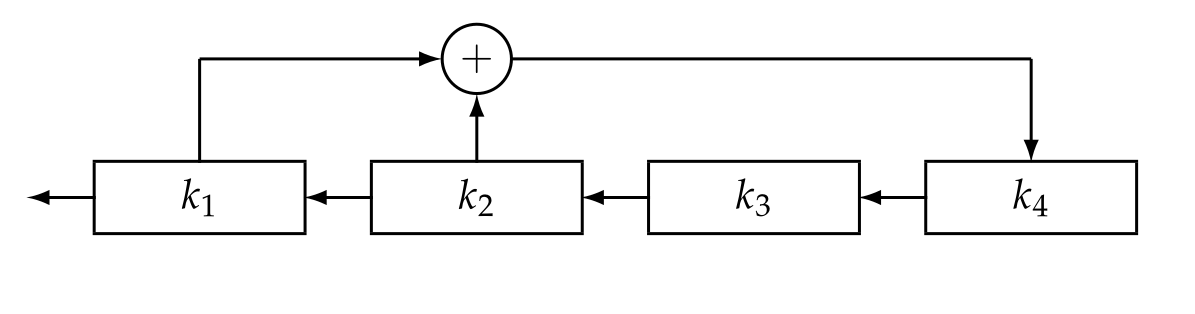
\includegraphics[scale=0.3]{Figures/Chapter2/lfsr.png}
    \caption{A linear feedback shift register.}
    \label{fig_1.4}
\end{figure}

\begin{definition}
    We define an \textbf{asynchronous stream cipher} to be a stream cipher whos
    keystream elements $z_i$ depend on the plaintext elements as well as the key
     $K$.
\end{definition}

\begin{definition}
    Let $\Pc=\Cc=\Kc=\faktor{\Z}{n\Z}$. Let $z_1=K \in \Kc$ and define
    $z_i=x_{i-1}$ for all $i \geq 2$. Then for  $0 \leq z \leq n$, define the
    \textbf{auto cipher} to be the pair $(e_z,d_z)$ such that $e_z:x \rightarrow
    x+z \mod{n}$ and $d_z:y \rightarrow y-z \mod{n}$.
\end{definition}

\begin{theorem}\label{1.1.10}
    The auto cipher defines a cryptosystem.
\end{theorem}
\begin{corollary}
    The auto cipher is an asynchronous stream cipher.
\end{corollary}
\begin{proof}
    Notice that given out key $K$,  $z_1=K$, and $z_i=x_{i-1}$ for all $i \geq
    2$. Thus taking  $z=z_1z_2 \dots$ to be our keystream, we see that $z$
    depends on $K$ and the elements $x_i$.
\end{proof}

We end the section with an example on the auto cipher.

\begin{example}
    Let $K=8 \mod{26}$ with plaintext \lstinline{rendezvous}. We first encode
    the plaintext with the map $q \rightarrow \faktor{\Z}{26\Z}$, $q_i
    \rightarrow i$ to get:
    \begin{equation*}
        17 \ 4 \ 13 \ 3 \ 4 \ 25 \ 21 \ 14 \ 20 \ 18
    \end{equation*}
    Then our keystream is
    \begin{equation*}
        8 \ 17 \ 4 \ 13 \ 3 \ 4 \ 25 \ 21 \ 14 \ 20
    \end{equation*}
    Applying $e_z$, we get
    \begin{equation*}
        25 \ 21 \ 17 \ 16 \ 7 \ 3 \ 20 \ 9 \ 8 \ 12
    \end{equation*}
    We then decode with the rule $\faktor{\Z}{26\Z} \rightarrow Q$ to get the
    ciphertext:
        \begin{verbatim}
                                ZVRQHDUJIM
        \end{verbatim}
    To decrypt, we take the encoded ciphertext and compute $x_1=d_8(25) \equiv
    17 \mod{26}, x_2=d_{17}(21) \equiv 4 \mod{26}, \dots, x_{10}=d_{20}(12)
    \equiv 18 \mod{26}$ which gives us the encoding: $17 \ 4 \ 13 \ 3 \ 4 \ 25
    \ 21 \ 14 \ 20 \ 18$ which gives us our original plaintext:
        \begin{verbatim}
                                rendezvous
        \end{verbatim}
\end{example}
